\documentclass{beamer}
\usepackage[utf8]{inputenc}
\usepackage{hyperref}
\usepackage{colortbl}
\usepackage{epstopdf}
\usepackage{graphicx}
\usepackage{mathtools}
\usepackage{listings}
\usepackage{letltxmacro}
\usepackage{algorithm, algpseudocode}

\renewcommand{\lstlistingname}{Listing}
\interfootnotelinepenalty=10000
\usepackage{listings}
\usepackage{algpseudocode}
\lstset{
    %numbers=left,
    numberblanklines=false,
    captionpos=b,
    breaklines=true,
    frameshape={RYRYN}{ny}{yn}{RYRYN},
    literate={~} {$\sim$}{1}
}

\usetheme{Madrid}
\usecolortheme{seagull}
\title[\fontsize{0.08cm}{1em}\selectfont Adversarial Hierarchical-Task Network para Jogos]{Adversarial Hierarchical-Task Network para Jogos em Tempo Real}
\author[Matheus de Souza Redecker]{Matheus de Souza Redecker
\\{\footnotesize Orientador: Prof. Dr. Felipe R. Meneguzzi}
}
\institute[PUCRS]{Pontificia Universidade Catolia do Rio Grande do Sul
\medskip\\
\url{matheus.redecker@acad.pucrs.br}
}
\date{\today}
\begin{document}

%---------------------------------------------------------------------------------

    \begin{frame}
        \titlepage
    \end{frame}

%---------------------------------------------------------------------------------
%	{
%	\setbeamercolor{background canvas}{bg=lightgray}
%    \begin{frame}{Outline}
%       	\begin{itemize}
%       		\item \textbf{Introduction and Motivation}
%       		\item \textbf{Background}
%       		\item \textbf{Extracting Recognition Information From Domain Analysis}
%			\item \textbf{Landmark-based Plan Recognition}
%			\item \textbf{Planning-based Plan Abandonment Detection}
%			\item \textbf{Experiments and Evaluation}
%			\item \textbf{Related Work}
%			\item \textbf{Conclusion}			
%        \end{itemize}
%    \end{frame}
%	}
%---------------------------------------------------------------------------------

%Motivação

\begin{frame}{Motivação}
	\begin{itemize}
	    \item Jogos em Inteligência Artificial
	    \item Algoritmo de Adversarial Hierarchical-Task Network
	    \item MicroRTS
    \end{itemize}
\end{frame}

%Background
{
	\setbeamercolor{background canvas}{bg=lightgray}
	\begin{frame}{Background}
		\vspace{5mm}
		\begin{itemize}
			\item \textbf{Busca}
			\item \textbf{Minimax}
			\item \textbf{Planejamento}       		
			\item \textbf{Planejamento Hierárquico}
		\end{itemize}
	\end{frame}
}
%BUSCA
\begin{frame}{Busca}
	\begin{itemize}
		\item Árvore das jogadas (\textit{game tree})
		\item Estado terminal
		\item Função de avaliação
		\item Busca Adversária
	\end{itemize}
	
	\begin{figure}[here]
		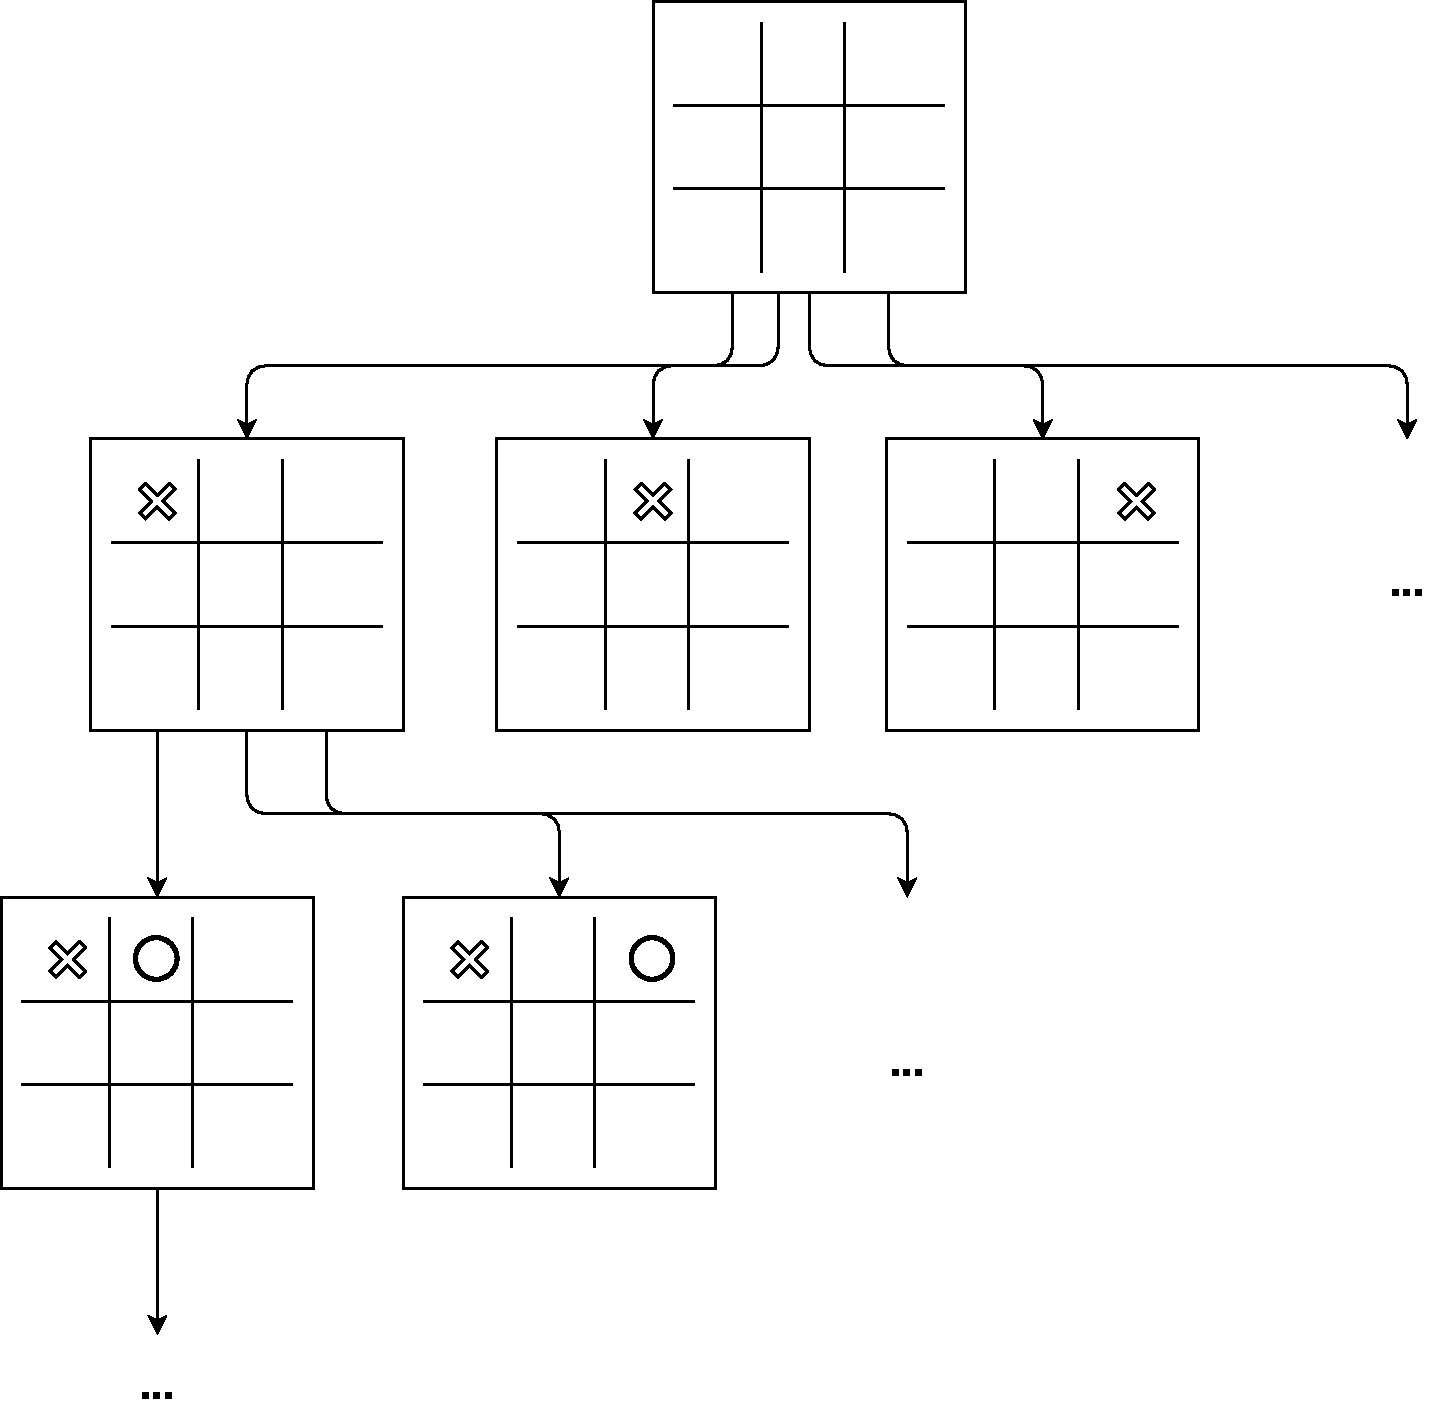
\includegraphics[width=0.45\linewidth]{fig/jogodavelha.pdf}	
	\end{figure}
\end{frame}
%Minimax
\begin{frame}{Minimax}
	\begin{itemize}
		\item Max
		\item Min
	\end{itemize}
	
	\vspace{-3mm}
	\begin{figure}[here]
		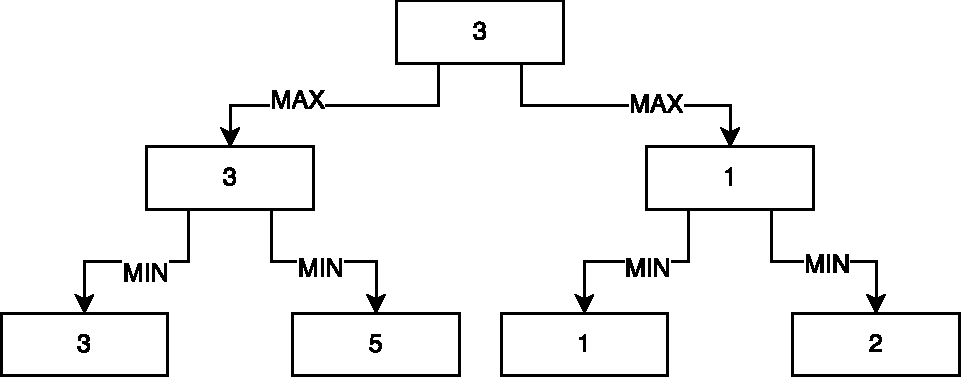
\includegraphics[width=0.8\linewidth]{fig/gametree.pdf}	
	\end{figure}	
\end{frame}

%Planejamento
\begin{frame}{Planejamento}
	
	\vspace{-3mm}
	\begin{figure}[here]
		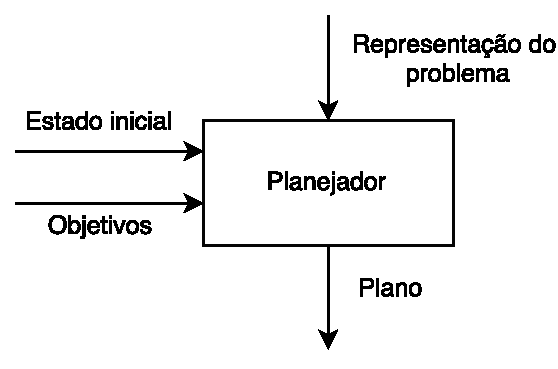
\includegraphics[width=0.6\linewidth]{fig/modelo.pdf}	
	\end{figure}	
\end{frame}
%Planejamento Hierárquico
\begin{frame}{Planejamento Hierárquico (HTN)}
	\begin{itemize}
		\item Tarefas alto nível
		\item Decomposições
	\end{itemize}
	\vspace{-3mm}
	\begin{figure}[here]
		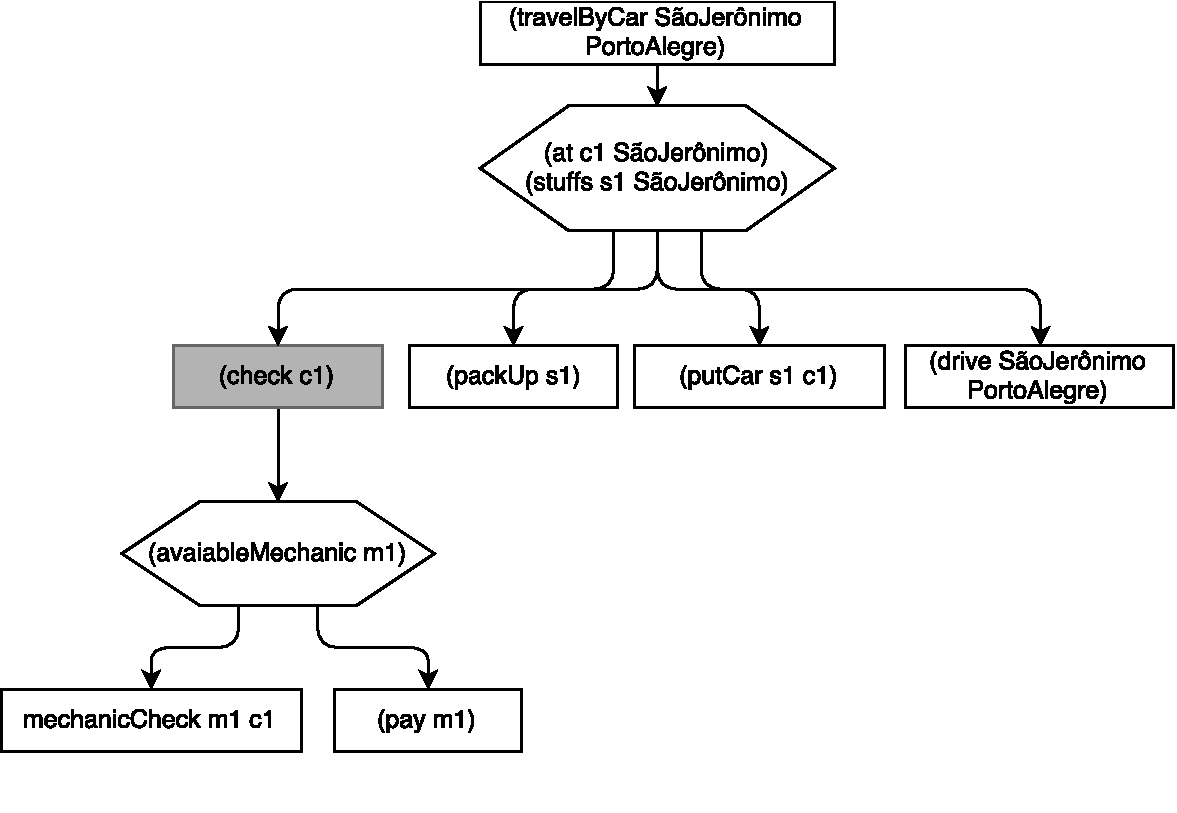
\includegraphics[width=0.7\linewidth]{fig/htnmethodresult.pdf}	
	\end{figure}	
\end{frame}
%Algoritmo de AHTN
\begin{frame}{Adversarial Hierarchical-Task Network}
	\begin{itemize}
		\item Como funciona o algoritmo?
		\item Minimax + planejamento hierárquico
	\end{itemize}
	
	{\tiny				
		\begin{algorithmic}[1]
				\Function {AHTNMax}{$s, N_{+}, N_{-}, t_{+}, t_{-}, d$}
				\If {$terminal(s) \vee d \leq 0$}\label{alg:lin:firstLine}
				\State	\Return $(N_{+}, N_{-}, e(s))$
				\EndIf
				\If {$nextAction(N_{+}, t_{+}) \neq \perp$} \label{alg:ahtn:nexaction}
				\State $t = nextAction(N_{+}, t_{+})$ 
				\State \Return $\Call{AHTNMin}{(\gamma(s,t), N_{+}, N_{-}, t, t_{-}, d-1)}$ \label{alg:ahtn:troca}
				\EndIf
				\State $N_{+}^{*} = \perp, N_{-}^{*} = \perp, v^{*} = -\infty$
				\State $\aleph = decompositions_{+}(s, N_{+}, N_{-}, t_{+}, t_{-})$ \label{alg:decompositions}
				\ForAll{$N \in \aleph$} \label{alg:ahtn:for}
				\State $(N^{'}_{+}, N^{'}_{-}, v^{'}) = AHTNMax(s, N, N_{-}, t_{+}, t_{-}, d)$
				\If{$v^{'} > v^{*}$}
				\State $N_{+}^{*} = N^{'}_{+}, N_{-}^{*} = N^{'}_{-}, v^{*} = v^{'} $
				\EndIf
				\EndFor		
				\State \Return $(N_{+}^{*}, N_{-}^{*}, v^{*} )$
				\EndFunction
		\end{algorithmic}
	}
\end{frame}

%MicroRTS+JSHOP2
{
	\setbeamercolor{background canvas}{bg=lightgray}
	\begin{frame}{Recursos Utilizados}
		\vspace{5mm}
		\begin{itemize}
			\item \textbf{MicroRTS}
			\item \textbf{JSHOP2}
		\end{itemize}
	\end{frame}
}
%MicroRTS
\begin{frame}{MicroRTS}
	\begin{itemize}
		\item O que é?
		\item Construções
		\item Unidades
		\item Técnicas de IA
	\end{itemize}
	\vspace{-3mm}
	\begin{figure}[here]
		\includegraphics[width=0.4\linewidth]{fig/microRTS.pdf}	
	\end{figure}	
\end{frame}
%JSHOP2
\begin{frame}{JSHOP2}
	\begin{itemize}
		\item Planejador
		\item Domínio
		\item Problema
	\end{itemize}
\end{frame}

{
	\setbeamercolor{background canvas}{bg=lightgray}
	\begin{frame}{Implementação}
		\vspace{5mm}
		\begin{itemize}
			\item \textbf{Ações do MicroRTS}
			\item \textbf{Modelagem do domínio}
			\item \textbf{Heurísticas}
			\item \textbf{Geração dos Planos}
			\item \textbf{Algoritmo AHTN}
		\end{itemize}
	\end{frame}
}

%Ações
\begin{frame}{Ações do MicroRTS}
	\begin{itemize}
		\item (diagrama com as ações)
	\end{itemize}
\end{frame}
%Modelagem do Domínio
\begin{frame}{Modelagem do Domínio}
	\begin{itemize}
		\item Unidade de ataque
		\item Operadores
		\item Métodos
	\end{itemize}
\end{frame}
%Heurística
\begin{frame}{Heurística}
	\begin{itemize}
		\item Unidades adversárias
		\item Estado terminal
	\end{itemize}
	\vspace{5mm}
	\begin{equation}
	h(s) =  (1*worker) + (5 * quartel) + (10 * base) + (2 * unidadesDeAtaque)
	\end{equation}
\end{frame}
%Geração dos Planos
\begin{frame}{Geração dos Planos}
	\begin{figure}[here]
		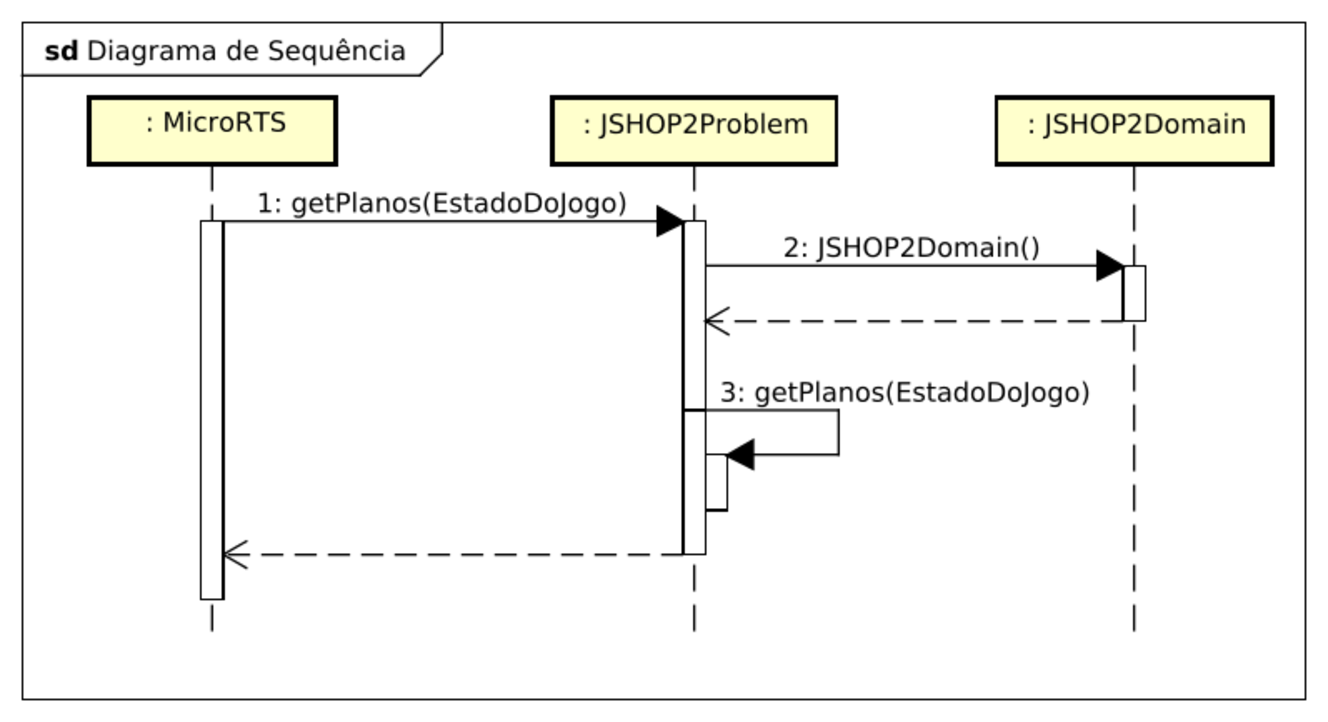
\includegraphics[width=0.9\linewidth]{fig/gerarPlano.pdf}	
	\end{figure}	
\end{frame}
%Implementação
\begin{frame}{Implementação}
	\vspace{5mm}
	{\footnotesize
	\begin{algorithmic}[1]		
		\Function {ATHNMax}{$estado, planoMax, planoMin, deph$}
		\If {$terminal(estado) \vee d \leq 0$} \label{alg:meuahtn:terminal}
		\State	\Return $(planoMax, planoMin, avaliacao(estado))$
		\EndIf
		\State {$nextAction(planoMax)$} \label{alg:meuahtn:nexaction}
		\State $(Pmax', Pmin', ev') = \perp, \perp, -\infty$
		\ForAll{$plano \in getPlanos(estado)$} \label{alg:meuahtn:for}
		\State $(Pmax, Pmin, ev) = \Call{AHTNMin}{(estado, planoMax, planoMin, deph-1)}$ \label{alg:meuahtn:ahtnmin}
		\If {$ev' > ev$} \label{alg:meuahtn:avali}
		\State $(Pmax', Pmin', ev') = (Pmax, Pmin, ev)$
		\EndIf		 		 		
		\EndFor
		\State \Return $(Pmax', Pmin', ev')$ \label{alg:meuahtn:retorno}
		\EndFunction
	\end{algorithmic}	
	}
\end{frame}

%Resultados
{
	\setbeamercolor{background canvas}{bg=lightgray}
	\begin{frame}{Resultados}
		\vspace{5mm}
		\begin{itemize}
			\item \textbf{Três mapas}
			\item \textbf{Tamanho das técnicas}
			\item \textbf{Tempo de geração das ações}
		\end{itemize}
	\end{frame}
}
%Mapa 1
\begin{frame}{Mapa 1}
	
	{\footnotesize
	\begin{tabular}{|c|cc|cc|}
		\hline
		\textbf{}           & \multicolumn{2}{c|}{\textbf{Domínio 1}}  & \multicolumn{2}{c|}{\textbf{Domínio 2}}  \\ \hline
		\textbf{Adversário} & \textbf{Lado Azul} & \textbf{Lado Vermelho} & \textbf{Lado Azul} & \textbf{Lado Vermelho} \\ \hline
		RandomIA            & 100\%              & 100\%                  & 100\%              & 100\%                  \\ \hline
		RandomBiasedIA      & 80\%               & 100\%                  & 100\%              & 100\%                  \\ \hline
		RangedRush          & 0\%                & 100\%                  & 100\%              & 100\%                  \\ \hline
		HeavyRush           & 0\%                & 100\%                  & 0\%                & 100\%                  \\ \hline
		LightRush           & 0\%                & 100\%                  & 0\%                & 100\%                  \\ \hline
		WorkerRush          & 0\%                & 0\%                    & 0\%                & 0\%                    \\ \hline
		MonteCarlo          & 60\%               & 80\%                   & 100\%              & 100\%                  \\ \hline
		Minimax             & 100\%              & 100\%                  & 100\%              & 100\%                  \\ \hline
		Portfolio           & 0\%                & 0\%                    & 0\%                & 0\%                    \\ \hline
	\end{tabular}
	}
\end{frame}
%Mapa 2
\begin{frame}{Mapa 2}
	
	{\footnotesize
			\begin{tabular}{|c|cc|cc|}
				\hline
				\textbf{}           & \multicolumn{2}{c|}{\textbf{Domínio 1}}  & \multicolumn{2}{c|}{\textbf{Domínio 2}}  \\ \hline
				\textbf{Adversário} & \textbf{Lado Azul} & \textbf{Lado Vermelho} & \textbf{Lado Azul} & \textbf{Lado Vermelho} \\ \hline
				RandomIA            & 100\%              & 100\%                  & 100\%              & 100\%                  \\ \hline
				RandomBiasedIA      & 40\%               & 80\%                   & 80\%               & 100\%                  \\ \hline
				RangedRush          & 0\%                & 100\%                  & 0\%                & 100\%                  \\ \hline
				HeavyRush           & 0\%                & 100\%                  & 0\%                & 100\%                  \\ \hline
				LightRush           & 0\%                & 100\%                  & 0\%                & 100\%                  \\ \hline
				WorkerRush          & 0\%                & 0\%                    & 0\%                & 0\%                    \\ \hline
				MonteCarlo          & 0\%                & 0\%                    & 0\%                & 0\%                    \\ \hline
				Minimax             & 0\%                & 100\%                  & 0\%                & 100\%                  \\ \hline
				Portfolio           & 0\%                & 60\%                  & 0\%                & 80\%                  \\ \hline
			\end{tabular}
	}
\end{frame}
%Mapa 3
\begin{frame}{Mapa 3}
	
	{\footnotesize
			\begin{tabular}{|c|cc|cc|}
				\hline
				\textbf{}           & \multicolumn{2}{c|}{\textbf{Domínio 1}}  & \multicolumn{2}{c|}{\textbf{Domínio 2}}  \\ \hline
				\textbf{Adversário} & \textbf{Lado Azul} & \textbf{Lado Vermelho} & \textbf{Lado Azul} & \textbf{Lado Vermelho} \\ \hline
				RandomIA            & 100\%              & 100\%                  & 100\%              & 100\%                  \\ \hline
				RandomBiasedIA      & 100\%              & 80\%                   & 100\%              & 80\%                   \\ \hline
				RangedRush          & 0\%                & 100\%                  & 0\%                & 100\%                  \\ \hline
				HeavyRush           & 0\%                & 100\%                  & 0\%                & 100\%                  \\ \hline
				LightRush           & 0\%                & 100\%                  & 0\%                & 100\%                  \\ \hline
				WorkerRush          & 0\%                & 0\%                    & 0\%                & 0\%                    \\ \hline
				MonteCarlo          & 0\%                & 0\%                    & 0\%                & 0\%                    \\ \hline
				Minimax             & 0\%                & 80\%                  & 80\%              & 80\%                   \\ \hline
				Portfolio           & 0\%                & 0\%                    & 0\%                & 0\%                    \\ \hline
			\end{tabular}
	}
\end{frame}
%Tamanho da IA
\begin{frame}{Tamanho das técnicas}
	
	{\footnotesize
		\begin{center}
			\begin{tabular}{|c|c|}
				\hline
				\textbf{Adversário}     & \textbf{Tamanho} \\ \hline
				Domínio HTN 1           & 19,9 kB          \\ \hline
				Domínio HTN 2           & 20,1 kB          \\ \hline
				RandomIA                & 4,0 kB           \\ \hline
				RandomBiasedIA          & 4,6 kB           \\ \hline
				RangedRush              & 13,7 kB          \\ \hline
				HeavyRush               & 14,0 kB          \\ \hline
				LightRush               & 14,0 kB          \\ \hline
				WorkerRush              & 13,6 kB          \\ \hline
				MonteCarlo              & 18,1 kB          \\ \hline
				Minimax                 & 12,9 kB          \\ \hline
				Portfolio               & 14,4 kB          \\ \hline
			\end{tabular}
		\end{center}
	}
\end{frame}
%Geração das ações
\begin{frame}{Tamanho das técnicas}
	\begin{figure}[here]
		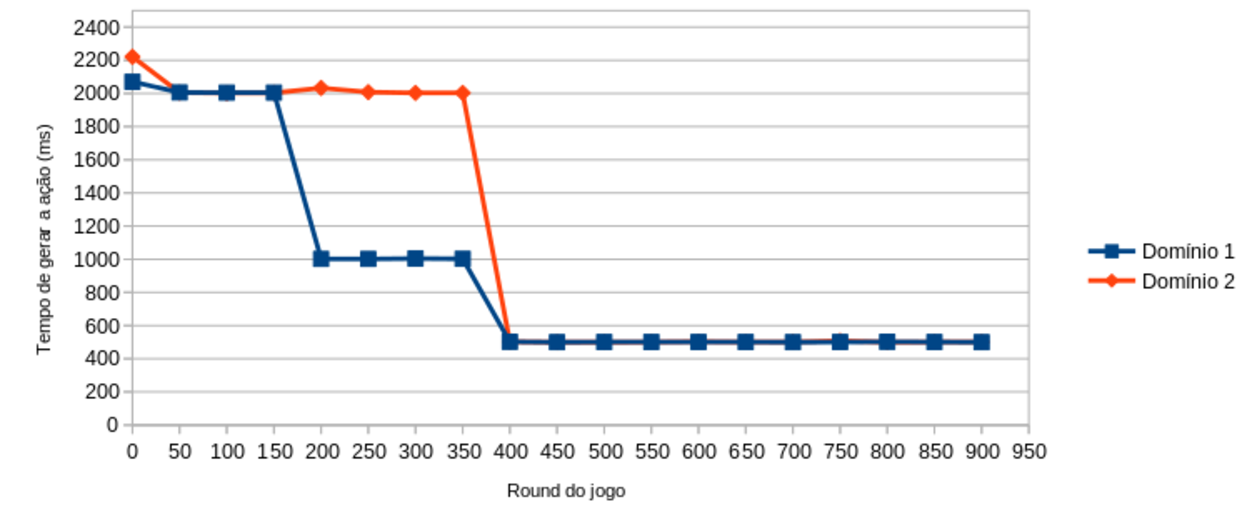
\includegraphics[width=0.9\linewidth]{fig/graph.pdf}
	\end{figure}
\end{frame}

%Conclusao
\begin{frame}{Conclusão}
	\begin{itemize}
		\item Problemas
		\item Influência do domínio
		\item Trabalhos futuros
	\end{itemize}
\end{frame}

%	{
%		\setbeamercolor{background canvas}{bg=lightgray}
%		\begin{frame}{}
%			\centering
%			Obrigado!
%		\end{frame}
%	}  


\end{document}